%%%%%%%%%%%%%%%%%%%%%%%%%%%%%%%%%%%%%%%%%%%%%%%%%%%%%%%%%%%%%%%%%%%%%%%%%%%%%%%%
%2345678901234567890123456789012345678901234567890123456789012345678901234567890
%        1         2         3         4         5         6         7         8

%\documentclass[letterpaper, 10 pt, conference]{orbieeeconfpre}  % Comment this line out if you need a4paper

\documentclass[a4paper, 10pt, journal]{wissarbIEEE}      % Use this line for a4 paper
%\conference{IEEE Conference for Awesome ORB Research}

\bibliographystyle{orbref-num}

\IEEEoverridecommandlockouts                              % This command is only needed if 
                                                          % you want to use the \thanks command

\overrideIEEEmargins                                      % Needed to meet printer requirements.

% See the \addtolength command later in the file to balance the column lengths
% on the last page of the document

\usepackage{hyperref}
\usepackage{graphicx}
\usepackage{tabularx}
\usepackage{booktabs}
\usepackage{lipsum}
%von Max eingebunden:
%\usepackage{times}
\usepackage{url}
\usepackage{hyperref}
\usepackage{amsmath}              % Matheamtische Formeln
\usepackage{amsfonts}             % Mathematische Zeichensätze
\usepackage{amssymb}              % Mathematische Symbole
%\usepackage{underscore}

%% Wo sind die Bilder?
%\graphicspath{{bilder/}}


% Eigenes Makro für Bilder
\newcommand{\bild}[3]{
\begin{figure}[h]
\centering
  \includegraphics[width=#2]{#1}
  \caption{#3}
  \label{#1}
\end{figure}}

\newcommand{\length}[1]{\lvert \vec{#1} \rvert}

\title{\LARGE \bf
Real time boid-simulations with shaders
}

\author{Maximilian Legnar and Prof. Dr. Rasenat}% <-this % stops a space

%\author{Maximilian Legnar$^{1}$ and Dr. Rasenat$^{2}$% <-this % stops a space
%
%\thanks{*Based on the guidelines published on the \href{http://conf.papercept.net/conferences/support/tex.php}{PaperCept conference manuscript management website}}% <-this % stops a space
%\thanks{$^{1}$Guybrush U. Threepwood is with the Institute for Pirate Sciences, Three-headed Monkey Group, University of  M\^el\'ee Island
%        {\tt\small gthreepwood@har.har-har.mi}}%
%\thanks{$^{2}$Alexander Schubert is with the Optimization in Robotics and Biomechanics Group, Institute of Computer Engineering, Heidelberg University, Berliner Str. 45, 69120 Heidelberg
%        {\tt\small alexander.schubert@ziti.uni-heidelberg.de, \href{http://orb.iwr.uni-heidelberg.de}{orb.iwr.uni-heidelberg.de}}}%
%}


\begin{document}



\maketitle

%%%%%%%%%%%%%%%%%%%%%%%%%%%%%%%%%%%%%%%%%%%%%%%%%%%%%%%%%%%%%%%%%%%%%%%%%%%%%%%%
\begin{abstract}

%...The goal is to show that ... This has been done by ..., it becomes clear that ...

%The purpose of this research is to develop a model for animal-like flocking simulations. The developed simulation-model is based on Reynolds boid-system \cite{Reynolds87flocks0}.

%Instead of treating the simulated flock like a particel-system, 

Basierend auf Reynolds Boid-System \cite{Reynolds87flocks} wird ein Modell für die Simulation von Tierschwärmen entwickelt. 
%Wesentlicher Fokus liegt dabei auf lebendig wirkende Schwarmbewegungen, interaktives Verhalten und Performance. 

Statt den simulierten Schwarm wie ein Partikelsystem zu behandeln, wird Reynolds Boid-Modell in ein Zellensystem, das mit den zellulären Automaten verwandt ist, transferiert. Diese Anpassung wird vorgenommen, damit die Simulation möglichst effizient von shader-Programmen ausgeführt werden kann.

Das Simulationsmodell unterteilt den Schwarm nicht in einzelne separate Individuen. Stattdessen ist der Schwarm eine im Raum ungleichmäßig verteilte Menge.
Der Schwarm wird daher als leuchtende Punkte-Wolke, von einer Textur dargestellt.

Die konzipierte Schwarmsimulation wird mittels Content-Driven Multipass Rendering prototypisch implementiert und in Echtzeit ausgeführt.

\end{abstract}

\section{Einleitung2}
Im Rahmen dieser Arbeit wird Reynolds Boid-Simulationsmodell so angepasst, dass alle für die Simulation nötigen Arbeitsschritte möglichst effizient von Shadern ausgeführt werden können.

Wegen der besonderen Funktionsweise von Shadern können manche Arbeitsschritte aus Reynolds Simulationsmodell nicht auf direktem Wege übernommen und implementiert werden. Daher werden manche Gesetzmäßigkeiten aus dem gegebenen Boid-Modell uminterpretiert und umformuliert. Bei Umformulierungen wird stets darauf geachtet, die grundlegenden Prinzipien des Boid-Systems möglichst unverändert zu lassen
%, da sich das dieses System bereits in der Praxis bewährt hat.

%Wie bereits erwähnt, ist CDMR die technische Grundlage für die Implementierung des Boid-Systems. Wesentliches Funktionsprinzip von CDMR ist die Bildung einer Shader-Pipeline, die Texturen verarbeitet. Also muss das Boid-System so uminterpretiert werden, dass dieses möglichst effizient von Texturen beschrieben und von Shadern simuliert werden kann.

%\ac{CDMR}


\section{Related work}

%Um die Bewegungen von Tierschwärmen zu simulieren, hat sich das sogenannte Boid-Modell von Reynolds etabliert. Auch in dieser Arbeit werden seine bekanntesten Werke, \cite{Reynolds87flocks} und \cite{Reynolds99steeringbehaviors}, als Fundament genutzt, um ein Modell für die Simulation aufzustellen.

In dieser Arbeit werden die grundlegenden Prinzipien von Reynolds, \cite{Reynolds87flocks} und \cite{Reynolds99steeringbehaviors}, aufgegriffen um ein neuartiges System zu modellieren, das besonders gut von Shadern und Texturen beschrieben werden kann.

Für gewöhnlich wird ein Boid-System wie ein Partikelsystem  behandelt \cite{Reynolds87flocks}, so wie in \cite{Oliver14Tschesche}. 
%In solch einem System ist jedes Individuum des Schwarms ein eigenständiges Objekt, das sich frei im Raum bewegen kann. 
In dieser Arbeit wird der Schwarm hingegen mithilfe eines Zellensystems beschrieben, in dem jede Zelle örtlich gebunden ist. Jede Zelle kann dabei von mehreren Individuen besucht werden. 
%Im Zellensystem befinden sich keine einzelnen Schwarmtiere, die eindeutig voneinander trennbar sind. Stattdessen  fließt  der Schwarm vielmehr, als zum Teil kontinuierlich zusammenhängende Menge, durch das Zellensystem. Das Zellensystem wird dabei von Texturen beschrieben.

%Der im Rahmen dieser Arbeit entstandene algorithmische Aufwand ist weniger von der Anzahl der simulierten Individuen abhängig, so wie es in \cite{Reynolds87flocks} der Fall ist. Stattdessen steigt hier der Rechenaufwand in Abhängigkeit von der Anzahl der verwendeten Zellen.

Reynolds Boid-System wird, wie in \cite{Oliver14Tschesche}, meist mithilfe von Grafikkartenschnittstellen wie \textit{OpenCV} oder \textit{CUDA} berechnet. In dieser Arbeit wird statt dessen auf die Verwendung von herkömmlichen Shadern gesetzt.

%Schwarmtiere werden für gewöhnlich als einzelne 3D-Modelle dargestellt. Beispielsweise als einzelne Fische \cite{Tu94artificialfishes:} oder Vögel  \cite{Oliver14Tschesche}.
%In dieser Arbeit erfolgt die Darstellung des Schwarms auf eine andere Weise. Einzelne Individuen sind hier kaum erkennbar, weil diese miteinander verschmelzen können. Der in Texturform hinterlegte Schwarm wird von Shadern als Punkte-Wolke dargestellt. Beispielsweise mittels \textit{Texture-Based Volume Rendering} \cite{GPUGems1}.  



\section{Method}
\subsection{Das Boid-System als Zellensystem}
\label{sec_noParticelCells}

Das Boid-System ist mit dem Partikelsystem verwand \cite{Reynolds87flocks} und kann daher für gewöhnlich auch als solches behandelt werden.

%Weil in diesem Fall das Boid-System von Texturen beschrieben wird, muss ein partikelähnliches System von Pixel-Shadern beschrieben werden. Herkömmliche Shader sind allerdings schlecht für die Beschreibung von Partikelsystemen geeignet. Das liegt an der folgenden Problematik:
 
Wesentlicher Bestandteil eines Partikelsystems ist die Bewegung, also die Positionsänderung, von Partikeln. 
Ein Shader kann ein Pixel allerdings nicht ohne weiteres bewegen. Das hängt damit zusammen, dass ein Pixel-Thread nicht in der Lage ist, Werte in andere Pixel zu schreiben. Jedes Pixel kann sein Rechenergebnis nur in sich selbst hinein schreiben.

%Jedes Pixel als einzelnes Partikel zu betrachten, ist daher nicht empfehlenswert. Ein Partikel, beschrieben von einem Pixel, könnte dann nämlich nicht ohne weiteres seine Position ändern und könnte sich somit schlecht bewegen.

Aufgrund dieser Einschränkung verabschieden wir uns an dieser Stelle vom Gedanken des Partikelsystems. Stattdessen wird das Boidsystem von einem Zellen-System beschrieben, wie bei shaderbasierten Flüssigkeitsströmungssimulationen \cite{GPUGems1} auch.

Das bedeutet, dass verwendete Texturen kein Partikelsystem, sondern ein Zellensystem repräsentieren. Ein Pixel aus einer Textur beschreibt kein umherfliegendes Boid, sondern eine Zelle, die eine reelle Menge von Boids, $D_i$, enthalten kann. Die Individuen des Schwarms bewegen sich dabei durch nebeneinanderliegende Zellen hindurch.

%Weil sich hinter jeder Zelle ein Pixel-Thread verbirgt, sind es im Grunde die Zellen, die die umherfliegenden Boids steuern.

\bild{bilder/Schwarmdarstellung}{5cm}{Left: A texture, that represents the boid-density, $D$. Each pixel is a real skalar value that represents the amount of boids, contained in this cell. Right: A texture, called $V$, that holds the control-vectors, $v$, for each cell. Each boid will follow its own control-vector}

In den nächsten Kapiteln werden Reynolds drei Grundverhaltensregeln, cohasion, seperation und alignment, umformuliert. Aus jeder Verhaltensregel werden sogenannte Steuervektoren, $\vec{v}$, generiert, wie in Abbildung \ref{bilder/Schwarmdarstellung} gezeigt. Die Summe aller Steuervektoren ergibt den Gesamtsteuervektor, $\vec{V}$, in dessen Richtung sich Boids bewegen.

%\section{Reynolds 3 Grundverhaltensregeln}


\subsection{Cohasion}

Das Steuersignal, das aus der Verhaltensregel der Kohäsion resultiert, wird $\vec{v}_c$ genannt. $\vec{v}_c$ ist vereinfacht gesagt ein Vektor, der zum Schwerpunkt aller gefundenen Nachbarn zeigt. 
Jede Zelle ist ein eigener Thread und berechnet ihr eigenes Kohäsions-Steuersignal, $\vec{v}_c$.
Um $\vec{v}_c$ zu berechnen, wird die Boid-Dichte-Textur, $D$, benötigt. $D$ gibt an, wie viele Boids in einer Zelle vorhanden sind.

Gegeben sei eine Zelle, $X$, die sich am Ort $x = (x_u \qquad x_v)$ befindet. Diese Zelle berechnet ein Kohäsions-Steuersignal für diesen Ort, $\vec{v}_c(x)$, mithilfe von $N$ gegebenen Wahrnehmungsvektoren. Mit einem Wahrnehmungsvektor, $\vec{s}_i$, kann eine Stichprobe, $D_i$, aus $D$ genommen werden.

\begin{equation}
D_i(x) = D(x + \vec{s}_i \cdot \frac{1}{R})
\label{Form_Di}
\end{equation}

%In Abbildung \ref{ChesionAbb} wird Zelle $X$ dargestellt, wobei in diesem Beispiel $N=4$ Wahrnehmungsvektoren gegeben sind.

\bild{bilder/ChesionAbb}{3cm}{Die rot markierte Zelle heißt $X$ und befindet sich an Position $x$. Sie besitzt 4 Wahrnehmungsvektoren, $\vec{s}_i$. Mit ihnen ist die Zelle in der Lage Stichproben, $D_i$, aus der Boid-Textur, $D$, zu entnehmen.}

Mithilfe der Stichproben, $D_i$, wird dann das Kohäsions-Steuersignal, $\vec{v}_c$, wie folgt berechnet:

\begin{equation}
\vec{v}_c(x) = \frac{\sum_{i=1}^N( \vec{s}_i \cdot D_i(x))}{\sum_{i=1}^N D_i(x)}
\label{Form_Cohesion}
\end{equation}

Im Zähler aus Gleichung \ref{Form_Cohesion}, wird im Grunde nichts geringeres getan, als Vektoren von der Zelle $X$ zu allen gefundenen Nachbarn zu spannen.

%Ist beispielsweise die Stichprobe $D_1$ aus Abbildung \ref{bilder/ChesionAbb} gleich 2, bedeutet dies, dass sich in der Zelle an der Stelle $x + \vec{s}_1$ zwei Boids befinden. Das Produkt aus $D_1$ und $\vec{s}_1$ ergibt $2 \cdot \vec{s}_1$. Somit werden zwei Vektoren zu einer Zelle gespannt, die zwei Boids aufbewahrt. Im Umkehrschluss Würden keine Vektoren nach $x + \vec{s}_1$ gespannt werden, wenn $D_1 = 0$ wäre, weil dann $D_1 \cdot \vec{s}_1 = 0$ ist.

Zum Schluss wird der Mittelwert aus allen gespannten Vektoren gebildet, indem durch die Anzahl aller gefundenen Nachbarn, $\sum_{i=1}^N D_i$, geteilt wird. 

%Mit Formel \ref{Form_Cohesion} wird $\vec{v}_c$ prinzipiell so wie Reynolds es in \cite{Reynolds99steeringbehaviors} vorschlägt, berechnet. Statt den Schwerpunkt der Nachbarn zu berechnen und dann einen Vektor von $x$ zum Schwerpunkt zu ziehen, kann auch der Durchschnitt aus allen zu den Nachbarn zeigenden Vektoren gebildet werden. Genau das wird hier getan. 


\subsection{Separation}

%Auch hier gilt wieder, das jeder Wahrnehmungsvektor, $\vec{s}_i$, eine Stichprobe, $D_i$, aus $D$ liefert, die ein Maß für die Anzahl der gefundenen Boids ist (Siehe Gleichung \ref{Form_Di}). Zudem wird wieder eine Zelle namens $X$, die sich bei Position $x$ befindet, betrachtet.

Das Separations-Steuersignal, $\vec{v}_s$, arbeitet im Gegensatz zur Kohäsion mit Vektoren, die von den entdeckten Nachbarn weg und zum gesteuerten Boid hin zeigen. Die Größe des Steuervektors, $\vec{v}_s$, steigt umso mehr an, je näher ein Nachbar ist. Reynolds empfiehlt hierfür mit umgekehrter Proportionalität zu arbeiten \cite{Reynolds99steeringbehaviors}.
So entsteht schlussendlich Formel \ref{Form_Separation}:

\begin{equation}
\vec{v}_s(x) = \sum_{i=1}^N (-D_i(x) \cdot e(\vec{s}_i) \cdot \frac{1}{\length{s_i}}) = - \sum_{i=1}^N(D_i(x) \cdot \frac{\vec{s}_i}{\length{s_i}^2})
\label{Form_Separation}
\end{equation}

Auch hier werden zuerst Vektoren zu allen Nachbarn gespannt, indem das Produkt aus $D_i$ und $\vec{s}_i$ gebildet wird. Weil in diesem Fall die Größe der gespannten Vektoren aber noch gesondert behandelt werden muss, werden sie vorerst normiert. So ergibt sich $D_i \cdot e(\vec{s}_i)$. 
%Wenn beispielsweise $D_i = 2$ ist, werden zwei Einheitsvektoren erzeugt, die von $x$ in die Richtung der beiden Nachbarn zeigen. 
Natürlich werden alle Einheitsvektoren noch umgedreht, damit abstoßende Kräfte entstehen. All diese abstoßenden Einheitsvektoren werden dann mit $1/ \length{s_i}$ gewichtet, so wie von Reynolds in \cite{Reynolds99steeringbehaviors} empfohlen. 
%Je kürzer $\vec{s}_i$ ist, desto größer wird die abstoßende Kraft sein. Zuletzt werden alle Vektoren summiert und es entsteht das fertige Separations-Steuersignal, $\vec{v}_s$.

\subsection{Alignment}
\label{subsec_Ausrichtung}

Das Steuersignal, $\vec{v}_a$, soll dafür sorgen, dass sich ein Boid der Bewegungsrichtung und Geschwindigkeit seiner Nachbarschaft anpasst. Diesmal ist also nicht nur die Menge, $D$, der Nachbarschaft von Interesse, sondern auch deren Bewegungsrichtungen, $\vec{V}$.

%Die Nachbarschaftssuche um Position $x$ herum, wird wieder mithilfe von $N$ Wahrnehmungsvektoren unternommen. Jeder Wahrnehmungsvektor, $\vec{s}_i$, wird dabei eine Stichprobe, $\vec{V}_i(x)$, aus der Textur, $\vec{V}$, entnehmen. 
%Die Berechnung von $\vec{V}_i(x)$ erfolgt nach Formel \ref{Form_Vi}:



%Wobei $R$ die Auflösung von $\vec{V}$ ist. 
%Hierbei ist zu beachten, dass $\vec{V}$ einen Steuervektor von einer Zelle liefert. 
In einer Zelle können sich mehrere Boids aufhalten. Das Bedeutet, dass $\vec{V}$ den Steuervektor von mehreren Boids repräsentieren könnte. Dies wird bei der Berechnung von $\vec{v}_a$, in Formel \ref{Form_Align}, berücksichtigt.

\begin{equation}
\vec{v}_a(x) = \dfrac{\sum_{i=1}^N(\vec{V}_i(x) \cdot D_i(x))}{\sum_{i=1}^N(D_i(x))} - \vec{V}(x)
\label{Form_Align}
\end{equation}

mit

\begin{equation}
\vec{V}_i(x) = \vec{V}(x + \vec{s}_i \cdot \dfrac{1}{R})
\label{Form_Vi}
\end{equation}

Zuerst wird im Zähler (Gleichung \ref{Form_Align}) des ersten Terms die Summe aller Steuervektoren aus der Nachbarschaft gebildet. 
%Die Summe aller Steuervektoren, aus einer benachbarten Zelle, kann mit $\vec{V}_i \cdot D_i$ errechnet werden. 
%Befinden sich beispielsweise zwei Boids in der durchsuchten Zelle, ist $D_i=2$. Dann müsste also das Steuersignal auch doppelt genommen werden um die Summe aller Steuersignale zu erhalten. Daher wird hier mit $\vec{V}_i \cdot D_i$ gearbeitet. 
Danach wird diese Summe durch die Anzahl an gefundenen Steuersignalen geteilt. Die Anzahl der gefundenen Steuersignale entspricht der Anzahl der gefundenen Boids, $\sum_{i=1}^N(D_i(x))$.

Nachdem die durchschnittliche Bewegungsrichtung der Nachbarschaft ermittelt wurde, wird davon die eigene Bewegungsrichtung, $\vec{V}(x)$, abgezogen, so wie es auch in \cite{Reynolds99steeringbehaviors} getan wird. 

%Formel \ref{Form_Align} kann auch zu Formel \ref{Form_AlignCa} vereinfacht werden. Bei dieser Vereinfachung wird ein Steuersignal aus einer Zelle, $\vec{V}_i$, direkt als Durchschnittssignal interpretiert.

%\begin{equation}
%\vec{v}_a(x)  \approx \dfrac{\sum_{i=1}^N(\vec{V}_i(x))}{N_V} - \vec{V}(x)
%\label{Form_AlignCa}
%\end{equation}

%Formel \ref{Form_AlignCa} unterscheidet sich von Gleichung \ref{Form_Align} in der Berechnung der durchschnittlichen Bewegungsrichtung. Hierfür werden alle Stichproben, $\vec{V}_i$, summiert und dann durch die Anzahl aller erfolgreichen Stichproben, $N_V$, geteilt.

%Formel \ref{Form_Align} berücksichtigt im Gegensatz zu Formel \ref{Form_AlignCa} wie voll eine durchsuchte Nachbarzelle ist. In Gleichung \ref{Form_Align} werden nämlich bei der Bildung des Mittelwertes Zellen, die mehr Boids enthalten, stärker gewichtet. Formel \ref{Form_AlignCa} hingegen gewichtet alle Stichproben gleich stark.

%\subsection{Definitionen und Vorschriften}
%\label{subsec_DefUVorschr}

%In diesem Kapitel wird festgelegt, wie sich eine Menge von Boids, $D(x)$, in Abhängigkeit eines gegebenen Steuervektors, $\vec{V}(x)$, bewegt und im Raum verteilt. Hierfür werden einige Definitionen festgelegt und Gesetze, die eingehalten werden müssen, vorgeschrieben.

\subsection{rules of boid movement}

%Die Bewegung der Boids wird in dieser Arbeit auch als \textit{Boid-Fluss} bezeichnet. Dieser Begriff beinhaltet den Gedanken, dass sich eine Menge Boids nicht sprunghaft bewegt, sondern vielmehr   fließt. Eine Menge Boids soll nicht in einem Moment von einer Zelle in eine andere  springen. Stattdessen sollen die Boids im übertragendem Sinne fließen und sich dabei gleichmäßig verteilen. Dadurch sollen natürlichere und flüssigere Bewegungen zustande kommen. 

%Würde immer der komplette Inhalt einer Zelle wandern, dann wäre auch immer dieselbe Menge Boids unterwegs. Nur beim Prinzip des Boid-Flusses kann sich der Inhalt einer Zelle auf mehrere Zellen verteilen, womit zu große Gruppenbildungen innerhalb einer Zelle vermieden werden können. Der Boid-Fluss soll sich auch vermischen können.

In order to find a formula, that discripe how the boids moves through the cell-system, we define following rules:

\subsubsection{Die Anzahl der Boids ist konstant}

Beim Transport der Boids sollte stets auf die Einhaltung des folgenden Gesetzes geachtet werden:

\begin{equation}
\sum_{i=1}^R \sum_{j=1}^R D(i,j)  = konstant
\label{Form_BoidFlussKonst}
\end{equation}

Formel \ref{Form_BoidFlussKonst} legt fest, dass die Anzahl aller vorhandenen Boids konstant bleiben muss. Die Anzahl soll im Verlaufe der Simulation weder sinken noch fallen. Beim Boid-Transport muss darauf stets geachtet werden.


\subsubsection{Ein Steuervektor entleert und befüllt dieselbe Menge Boids}
\label{subsubsec_D_V}

Gegeben sei eine Zelle $X$ bei $x$. Sie besitzt einen Steuervektor $\vec{V}$ und $D$ Boids.

Der Steuervektor, $\vec{V}$, verursacht den Transport einer Menge Boids, $D_V$, wobei \\ $D_V <= D$ (damit Gesetz \ref{Form_BoidFlussKonst} eingehalten wird).

Durch den Transport verliert Zelle $X$ $D_V$ Boids, während genau dieselbe Menge in ihrer Umgebung verteilt wird. Die Menge $D_V$ wird auf $N$ andere Zellen verteilt, diese Zellen werden als \textit{besuchte} Zellen bezeichnet. Jede besuchte Zelle bekommt eine Teilmenge von $D_V$, namens $D_{Vi}$ gutgeschrieben.

\bild{bilder/LeafEqEnter}{8.5cm}{Es werden drei unterschiedliche Verteilungsarten gezeigt. Die rot markierte Zelle verteilt Boids in Richtung von $V$. Die Verteilende Zelle verliert dabei $D_V$ Boids. Genau diese Menge wird dann in die orange markierten Zellen verteilt. Hierfür können unterschiedliche Verteilungsarten konzipiert werden.}

Die Summe aller $N$ Teilmengen, $D_{Vi}$, muss genau so groß sein, wie die verloren gegangene Menge $D_V$.

\begin{equation}
\sum_{i=1}^N(D_{V_i}) = D_V
\label{Form_SummeD_V_i}
\end{equation}

Für die Verteilung von $D_V$ können, so wie in Abbildung \ref{LeafEqEnter} vorgeschlagen, unterschiedliche Verteilungsmethoden eingesetzt werden. $D_{Vi}$ kann einer einzigen Zelle überreicht oder auf mehrere Zellen verteilt werden.

%Bei der Verteilung muss aber immer Gleichung \ref{Form_SummeD_V_i} erfüllt sein. Außerdem sollten die Teilmengen, $D_{Vi}$, sinngemäß in Richtung des Steuervektors, $\vec{V}$, verteilt werden, damit sich die Boids in die angestrebte Richtung bewegen.


\subsubsection{Maximale Bewegungsreichweite eines Boids}

Bei der Advektion von Texturen sollte ein Pixel pro Zeitschritt nicht weiter als eine Pixellänge bewegt werden. Ansonsten können Instabilitäten entstehen, wodurch sich die bewegte Textur, laut \cite{GPUGems1}, explosionsartig aufblähen kann.

Daher sollte bei der Simulation darauf geachtet werden, dass ein Boid pro Simulationsschritt keine Zelle überspringt. Diese Regel sollte bei der Konzipierung von Verteilungsmethoden berücksichtigt werden. Verteilungsmethoden wie die Methode, die in Abbildung \ref{LeafEqEnter} ganz rechts zu sehen ist, sollten daher vermieden werden.



\subsection{Boid-movement formula}
Nachdem in Kapitel \ref{subsec_DefUVorschr} festgelegt wurde, nach welchen Gesetzen und Formeln sich der Schwarm im Zellensystem verteilen soll, kann eine allgemein gültige Formel für den Transport von $D$ aufgestellt werden.

Grundsätzlich geben Zellen pro Simulationsschritt Boids an Nachbarzellen ab und nehmen neue Boids von ihren Nachbarn auf. Dieser Prozess kann über Formel \ref{Form_AdvektUeberischt} ausgedrückt werden:

\begin{equation}
D(x,t+dt) = D(x,t)-D_{leave}(x,t) + D_{enter}(x,t)
\label{Form_AdvektUeberischt}
\end{equation}

In Gleichung \ref{Form_AdvektUeberischt} aktualisiert eine Zelle, die sich bei $x$ befindet, ihre Boids. Hierfür wird $D_{leave}(x,t)$ von $D(x,t)$ abgezogen und $D_{enter}(x,t)$ zu $D(x,t)$ addiert.

Zunächst wird es darum gehen, den bis jetzt unbekannten Termen  $D_{leave}$ und $D_{enter}$ näher zu kommen.



%\subsubsection{Verlassene Zellen}
%\label{subsec_VerlasseneZellen}
Gegeben sei eine Zelle $X$ am Ort $x$. Sie besitzt $D(x)$ Boids. Außerdem besitzt sie einen Steuervektor, $\vec{V}(x)$, für ihre Boids. $\vec{V}(x)$ repräsentiert den derzeitigen  Bewegungswunsch der in $X$ enthaltenen Boids. Im Steuervektor ist auch die Information enthalten, wie viele Boids aus der Zelle fließen werden, $D_{leave}(x)$. Die Länge des Steuervektors stellt dabei die Dringlichkeit des Bewegungswunsches dar. Ist $\vec{V}(x)$ groß, haben es die Boids im übertragendem Sinne eilig. 
%Vielleicht weil gerade die Gefahr besteht den Anschluss zum Schwarm zu verlieren, weil ein Jäger in der Nähe ist, oder weil eine Kollisionsgefahr mit benachbarten Boids besteht. Deswegen sollte die Menge der Boids, die die Zelle verlassen, $D_{leave}(x)$, mit $\length{V(x)}$ wachsen.

\begin{equation}
D_{leave}(x) \thicksim \length{V(x)}
\label{Form_DLeavePropV}
\end{equation}

Außerdem ist $D_{leave}(x)$ neben $\length{V(x)}$ auch abhängig von $D(x)$. $D_{leave}(x)$ ist schließlich eine Teilmenge von $D(x)$, wobei $D_{leave}(x) <= D(x)$.

Daraus ergibt sich schlussendlich die finale Formel für $D_{leave}(x)$:

\begin{equation}
D_{leave}(x) = \length{V(x)} \cdot D(x)
\label{Form_DLeaveFinal}
\end{equation}

Außerdem muss dabei stets Gleichung \ref{Form_lengthVOne} erfüllt sein, damit $D_{leave}(x) <= D(x)$ gilt.

\begin{equation}
\length{V(x)} <= 1
\label{Form_lengthVOne}
\end{equation}

Bei der Generierung der Steuersignale sollte also stets darauf geachtet werden, das ein Steuervektor niemals größer als 1 wird.

An dieser Stelle sollte die folgende Erkenntnis nicht fehlen: Die transportierte Menge, $D_V$, ist genauso groß wie die verlorene Menge, $D_{leave}$.

\begin{equation}
D_{leave}(x) = D_V(x)
\label{Form_DLeaveEqDV}
\end{equation}


%\subsubsection{Zellenbesuch}
%\label{sec_Zellenbesuch}

Wie $D_{Enter}$ berechnet wird, hängt davon ab, nach welchem Verteilungsgesetz die transportierte Menge, $D_V$, verteilt wird. 
%Im Rahmen dieser Arbeit wurden zwei Verteilungsmethoden entwickelt und ausgetestet.

%Bei beiden Methoden findet der Boid-Austausch immer zwischen direkt benachbarten Zellen statt. Pro Simulationsschritt kann ein Boid also keine Zelle überspringen, was zu stabilen Simulationsergebnissen führen soll.


%\subsubsection{Verteilung in eine Nachbarzelle}

Ein besonders einfaches Verteilungsgesetz ist die Verteilung der Menge $D_V$ in eine Nachbarzelle. Diese Methode bringt dabei den Vorteil eines geringen Rechenaufwands mit sich.

%Solange $\length{V}$ kleiner als 1 ist, kommt auch bei dieser einfachen Methode ein Boid-Fluss zustande, weil dann nur ein Teil von $D$ in eine benachbarte Zelle fließen kann.

%Es folgt anhand eines Beispiels die Beschreibung des festgelegten Verteilungsgesetzes:

%Gegeben sei eine Zelle, $X$, die sich an der Position $x=(u_x \qquad v_x)$, in einem zweidimensionalem Zellensystem befindet. Ihr Steuervektor, $\vec{V}(x)$, zeigt ungefähr auf die obere, rechte Nachbarzelle von $X$. $\vec{V}(x)$ sei also ungefähr $(1 \qquad -1)$.

%\bild{bilder/VerteilungInEineNachbarzelle}{7cm}{Auch wenn $V$ nicht exakt auf die orange markierte Zelle zeigt, bekommt diese 100\% von $D_V$ gut geschrieben.}

%Die Zelle $X$ wird dann $D_{leave}(x) = D_V(x)$ (Siehe Formel \ref{Form_DLeaveFinal}) Zellen verlieren und an die Nachbarzelle, auf die $V(x)$ zeigt, abgeben. Der Zelle, die sich bei $x + (1 \qquad -1)$ aufhält, werden dann $D_V(x)$ Boids gutgeschrieben.

%Aufgrund der Funktionsweise von Shadern kann eine Zelle, $X$, keine Werte in eine Nachbarzelle schreiben. Sie kann daher $D_V(x)$ nicht an ihre Nachbarzelle übergeben. Stattdessen müsste die Nachbarzelle selbst   erkennen, dass der Steuervektor $\vec{V}(x)$ von Zelle $X$ auf sie selbst zeigt. Denn nur die Nachbarzelle selbst, kann $D_V(x)$ zu ihren Boid-Bestand hinzufügen.

Eine Zelle, $X$, muss all Ihre direkten Nachbarn durchsuchen, um in Erfahrung zu bringen, ob Steuervektoren aus ihrer Nachbarschaft auf sie selbst zeigen. Die Nachbarsuche kann mithilfe von unterschiedlich orientierten Testvektoren, $\vec{T}_i$, erfolgen, so wie in Abbildung \ref{AdvektVergleichsvektoren} dargestellt.

\bild{bilder/AdvektVergleichsvektoren}{8.5cm}{Die rot eingefärbte Zelle untersucht ihre Nachbarschaft mit $N_c$ Testvektoren, $T_i$. Die Testvektoren repräsentieren auch die möglichen Bewegungsrichtungen die ein Boid einschlagen kann. Wenn nur 4 Testvektoren verwendet werden, heißt das auch, dass sich die Boids in nur 4 unterschiedliche Richtungen bewegen können.}

%%%%%%%%%%%%%%%%%%%%%%%%%%%%%
%Jeder Testvektor heißt $\vec{T}_i$ und ist normiert. In Abbildung \ref{AdvektVergleichsvektoren} werden $N_c=8$ Testvektoren eingesetzt. Die Position einer durchsuchten Nachbarzelle ist $x+\vec{T}_i/R$. $R$ ist die Auflösung der verwendeten Texturen.
%
%Ob eine Nachbarzelle von Zelle $X$ auf Position $x$ zeigt, kann herausgefunden werden, indem mit Vergleichsvektoren, $\vec{c}_i$, gearbeitet wird.
%
%Eine Nachbarzelle, die sich bei $x+\vec{T}_i \dfrac{1}{R}$ befindet, 
%%liefert eine Boid-Dichte, $D_i=D(x+\vec{T}_i \dfrac{1}{R})$, einen Steuervektor, $\vec{V}_i=\vec{V}(x+\vec{T}_i  \dfrac{1}{R})$ und 
%bekommt einen Vergleichsvektor, $\vec{c}_i$ zugeordnet. Eine Nachbarzelle liefert eine Boid-Dichte namens $D_i=D(x+\vec{T}_i \dfrac{1}{R})$ und einen Steuervektor namens $\vec{V}_i=\vec{V}(x+\vec{T}_i  \dfrac{1}{R})$.
%
%\bild{bilder/AdvektVergleichEineZelle}{7cm}{Der Steuervektor, $\vec{V}_i$, des rechten Nachbars von $X$, muss in die selbe Richtung wie $\vec{c}_i$ zeigen, damit es zu Boid-Austausch kommt. Dabei ist eine maximale Toleranz von $\beta/2$ erlaubt. In diesem Fall zeigt $\vec{V}_i$ in eine andere Richtung, daher wird es nicht zum Boid-Austausch kommen.}
%
%$\vec{c}_i$ ist ein normierter Vektor, der genau von der Nachbarzelle auf Zelle $X$ zeigt. Für $\vec{c}_i$ gilt:
%
%\begin{equation}
%c_i = -T_i
%\label{Form_CiEqTi}
%\end{equation}
%
%In Abbildung \ref{AdvektVergleichEineZelle} vergleicht die Zelle $X$ den Steuervektor einer Nachbarzelle, $\vec{V}_i$, mit $\vec{c}_i$. Hierfür wird ein Vergleichswinkel namens $\beta$, verwendet.  $\beta$ setzt sich wie folgt zusammen:
%
%\begin{equation}
%\beta = \dfrac{2 \pi}{N_c} \qquad N_c = [4 \qquad 8]
%\label{Form_Beta}
%\end{equation}
%
%Wobei $N_c$ die Anzahl der durchsuchten Nachbarzellen ist.
%
%Nur wenn der Winkel zwischen $\vec{V}_i$ und $\vec{c}_i$ kleiner als $\beta/2$ ist, kommt es zum Boid-Austausch zwischen den beiden Zellen aus Abbildung \ref{AdvektVergleichEineZelle}. Der Winkel zwischen den beiden Vektoren heißt $\alpha$, wobei $0 < \alpha < \pi$. Weil $\vec{c}_i$ ein normierter Vektor ist, gilt:  
%
%\begin{equation}
%e(\vec{V}_i) \cdot \vec{c}_i = \cos{\alpha}
%\end{equation}
%
%Die Bedingung $\alpha < \beta/2$ ist immer dann erfüllt wenn:
%
%\begin{equation}
%e(\vec{V}_i) \cdot \vec{c}_i > \cos{(\beta/2)} 
%\label{Form_AdvektBetaVergleich}
%\end{equation}
%
%Immer wenn Gleichung \ref{Form_AdvektBetaVergleich} erfüllt ist, war der Vektorvergleich erfolgreich und es kommt zum Boid-Austausch zwischen den beiden Zellen.  
%%%%%%%%%%%%%%%%%%%%%%%%%%%%%%%%%%%%%%%%%%%%%%%%%%%%%%

%Für die Boid-Aufnahme wird Zelle $X$ die Menge der vom Nachbar ausgesendeten Boids, $D_{Enter_i}$, berechnen, um genau diese Menge aufzunehmen. 
Stellt sich heraus, dass ein benachbarter Steuervektor auf Zelle $X$ zeigt, nimmt Sie $D_{Enter_i}$ Zellen vom Nachbar auf.

\begin{equation}
D_{Enter_i} = D_{Leave}(x+\dfrac{\vec{T}_i}{R}) = D(x+\dfrac{\vec{T}_i}{R}) \cdot |\vec{V}(x+\dfrac{\vec{T}_i}{R})| 
\label{Form_D_V_Nachbar}
\end{equation}

Nachdem Zelle $X$ all ihre $N_c$ Nachbarn untersucht hat, sind $n_c$ Nachbarzellen bekannt, die ihre Boids an $X$ abgeben. Es gilt $0<=n_c<=N_c$. Aus jedem, der $n_c$ Nachbarn, entsteht ein $D_{Enter_i}$. Zelle $X$ nimmt dann insgesamt $D_{Enter}(x)$ Boids aus ihrer Nachbarschaft auf:

\begin{equation}
D_{Enter}(x) = \sum_{i=1}^{n_c} ( D_{Enter_i})
\label{Form_D_EnterFinal}
\end{equation}

%Um individuellere Bewegungen zu erhalten, lohnt es sich, alle 8 zur Verfügung stehenden Nachbarn durchzusuchen. Dann ist $N_c=8$. Das bedeutet, dass sich ein Boid pro Zeitschritt in eine von 8 unterschiedlichen Bewegungsrichtungen bewegen kann. Nämlich in die Richtungen, in die die 8 eingesetzten Testvektoren zeigen. 
%Es kann aber auch festgelegt werden, dass sich ein Boid nur in eine der 4 Richtungen $\vec{T}_1=(1 , 0)$, $\vec{T}_2=(-1,0)$, $\vec{T}_3=(0,1)$ oder $\vec{T}_4=(0,-1)$ bewegen kann. Dann wäre $N_c=4$ und der Vergleichswinkel $\beta/2$ größer.

%
%
%\subsubsection{Verteilung in zwei Zellen}
%
%Bei dieser Verteilungsmethode verteilt ein Steuervektor seine transportierte Menge, $D_V$, in zwei benachbarte Zellen. 
%
%Betrachtetet wird wieder eine Zelle, namens $X$, bei position $x$. Ihr eigener Steuervektor, $\vec{V}$, entzieht ihr wie immer eine Menge Boids, $D_V = D_{Leave}$. Die Menge, $D_V$, wird daraufhin in zwei Nachbarzellen, $X_1$ und $X_2$, verteilt. Dabei erhält Zelle $X_1$ $D_{V1}$ Boids und Zelle $X_2$ $D_{V2}$ Boids.
%
%Abbildung \ref{EnterSmoothIdea} visualisiert diese Art der Verteilung von $D_V$.
%
%\bild{bilder/EnterSmoothIdea}{4cm}{Bei der Verteilungsmethode \textit{Verteilung in zwei Zellen }verteilt die rot markierte Zelle, $X$, ihre Menge, $D_V$, in zwei Nachbarzellen (orange). }
%
%Bei der Verteilung der beiden Teilmengen  muss Gesetz \ref{Form_SummeD_V_i} erfüllt werden. Daher muss für die beiden Teilmengen gelten (siehe Formel \ref{FormTVTeilmengen}):
%
%\begin{equation}
%D_V = D_{V1} + D_{V2} 
%\label{FormTVTeilmengen}
%\end{equation}
%
%Formel \ref{FormTVTeilmengen} kann weiter aufgeschlüsselt werden in Gleichung \ref{FormTVTeilmengen2}:
%
%
%\begin{equation}
%D_V = m_1 \cdot D_V + m_2 \cdot D_V \qquad m_1 + m_2 = 1
%\label{FormTVTeilmengen2}
%\end{equation}
%
%Die beiden Faktoren $m_1$ und $m_2$ geben die Anteile an, die von $D_V$ entzogen und in Zelle $X_1$ und $X_2$ fließen sollen. Die summe aus $m_1$ und $m_2$ muss 1 sein, damit Gleichung \ref{FormTVTeilmengen} erfüllt wird.
%
%Bei der Aufteilung von $D_V$ zwischen den beiden Zellen $X_1$ und $X_2$ gilt folgende Regel: Die Zelle, auf die $\vec{V}$ eher zeigt, bekommt mehr von $D_V$ ab, als die andere Zelle. Zeigt $\vec{V}$ exakt auf $X_1$, bekommt $X_1$ $100\%$ von $D_V$ und $X_2$ bekommt nichts. Dann wäre $m_1=1$ und $m_2=0$. Zeigt $\vec{V}$ genau zwischen $X_1$ und $X_2$, bekommen beide Zellen gleichviel von $D_V$. Dann wäre $m_1=m_2=0,5$.
%
%Auch hier muss wieder eine Zelle $N_c$ Nachbarzellen untersuchen, um selbst herauszufinden, ob Nachbarzellen Boids abgeben wollen. Dabei kann, genau wie im vorigem Kapitel auch, mit normierten Testvektoren, $\vec{T}_i$, gearbeitet werden, die zu den Nachbarzellen zeigen. Der Steuervektor einer Nachbarzelle heißt wieder $\vec{V}_i$. $\vec{V}_i$ wird wieder mit einem Vergleichsvektor, $\vec{c}_i = -\vec{T}_i$ verglichen. Beim Vergleich wird der Winkel, $\alpha$, zwischen $\vec{V}_i$ und $\vec{c}_i$ betrachtet (siehe Abbildung \ref{VertIn2ZellenAlpha}).
%
%\bild{bilder/VertIn2ZellenAlpha}{7cm}{Zelle $X$ wird, je nachdem wie klein $\alpha$ ist, einen prozentualen Anteil von $D_{Vi}$ abbekommen. Der restlichen Teil wird in eine andere Zelle verteilt werden. In diesem Fall wird die Zelle, die sich unten rechts von $X$ befindet, einen größeren Anteil von $D_{Vi}$ bekommen als $X$.}
%
%Der Winkel $\alpha$ wird mit einem Winkel, $\beta = \dfrac{2 \pi}{N_c}$, verglichen. In Abbildung \ref{VertIn2ZellenAlpha} ist $\beta = \pi/2$, weil hier  $N_c=4$ gilt. Wenn $\alpha = 0$ ist, zeigt der Steuervektor des Nachbars genau auf Zelle $X$ und die Nachbarzelle wird $100\%$ von ihrer Menge, $D_V$, an $X$ abgeben. Wenn $\alpha \geq \beta$ ist, fließen keine Boids vom Nachbar zu $X$. Wenn $\alpha$ zwischen 0 und $\beta$ liegt, zeigt der Steuervektor der Nachbarzelle ungefähr in Richtung von $X$ und es wird der Anteil, $m_i \cdot D_{Vi}$ aus der Nachbarzelle zu $X$ fließen. $m_i$, soll eine lineare Funktion von $\alpha$ sein. Der Funktionsverlauf soll wie in Abbildung \ref{VertIn2ZellenFunktionModellierung} gezeigt, verlaufen: 
%
%\bild{bilder/VertIn2ZellenFunktionModellierung}{9cm}{$m_i$ als Funktion von $\alpha$. Sie muss linear sein, damit $D_{Vi}$ richtig aufgeteilt wird. Bekommt eine Zelle beispielsweise $70\%$, wird eine andere Zelle $30\%$ von $D_{Vi}$ ernten.}
%
%Mithilfe von Abbildung \ref{VertIn2ZellenFunktionModellierung} kann die gesuchte Funktion, $m_i$ von $\alpha$, aufgestellt werden:
%
%\begin{equation}
%m_i = - \dfrac{1}{\beta} \cdot \alpha + 1 \qquad m_i(\alpha \geq \beta)=0
%\label{Form_mi}
%\end{equation}
%
%Formel \ref{Form_mi} ist von $\alpha$ abhängig. $\alpha$ ist der Winkel zwischen $\vec{c}_i$ und $\vec{V}_i$ und kann mit dem Skalarprodukt ermittelt werden. So wie Formel \ref{Form_alpha2Zellen} zeigt:
%
%\begin{equation}
%\alpha = \arccos{( \vec{c}_i \cdot e(\vec{V}_i) )}
%\label{Form_alpha2Zellen}
%\end{equation}
%
%Zelle $X$ berechnet für jeden der $N_c$ Nachbarn ein $m_i$ und nimmt dann von jeder Nachbarzelle $m_i \cdot D_{Vi}$ Boids auf. $D_{Vi}$ ist die Menge Boids, die ein Nachbar verliert. Somit kann die finale Formel für die Verteilung in zwei Zellen gebildet werden (siehe Gleichung \ref{Form_Vert2ZellenFinal}):
%
%\begin{equation}
%D_{Enter}(x)=\sum_{i=1}^{N_c}(m_i \cdot D(x+\vec{T}_i \cdot \dfrac{1}{R}) \cdot |\vec{V}(x+\vec{T_i} \cdot \dfrac{1}{R})|  )
%\label{Form_Vert2ZellenFinal}
%\end{equation}
%
%Voraussetzung für Formel \ref{Form_Vert2ZellenFinal} ist, das die Testvektoren, $\vec{T}_i$, gleichmäßig und rotationssymmetrisch um $X$ herum verteilt sind und immer in Richtung Zentrum einer Zelle zeigen. Hierfür wird die Verwendung des folgenden Testvektorsets empfohlen: 
%
%$\vec{T}_1=(1 , 0)$, $\vec{T}_2=(-1,0)$, $\vec{T}_3=(0,1)$ und $\vec{T}_4=(0,-1)$.




\section{Evaluation}


%Im Rahmen dieser Arbeit konnten fast alle gesetzten Ziele erreicht werden. Anhand des konzipierten Simulationsmodells konnte ein Prototyp implementiert werden, der fast alle Anforderungen aus Kapitel \ref{sec_Anforderungen} erfüllt. 

Der im Prototyp simulierte Schwarm kann durch Einsatz einfacher Zusatzverhaltensregeln von einem menschlichen Spieler gejagt oder verfolgt werden. 
Die Bewegungen des Schwarms können bei entsprechender Parametrisierung realistisch und lebendig gestaltet werden. Ohne mit zufällig generierten Steuervektoren arbeiten zu müssen, bewegen sich manche Schwärme scheinbar in zufällige Richtungen, als ob die virtuellen Lebewesen ein eigenes Ziel verfolgen würden.

Die Performance des implementierten Prototyps erwies sich, entgegen aller Erwartungen, als überraschend gut. Die Messungen aus Kapitel \ref{sec_performance} lassen vermuten, dass sich das konzipierte Simulationsmodell durchaus in der Praxis anwenden lässt. Künftige Videospiele könnten von diesen interaktiven Schwarm-Wesen profitieren, zumal sich die entwickelte Simulation von herkömmlichen Shadern ausgeführt werden kann. Shader-Programme, die mithilfe der Unreal Engine 4 implementiert wurden, lassen sich ohne große Umstände auf einige Plattformen portieren. 
%Von allen handelsüblichen Konsolen, bis hin zu Smartphones. Smartphone-Besitzer mithilfe des Touchscreens mit dem Schwarm interagieren zu lassen, ist durchaus umsetzbar. 

%Der erstellte Prototyp konnte aus zeitlichen Gründen nur als zweidimensionale Schwarmsimulation implementiert werden. Die Idee, den virtuellen Schwarm als dreidimensionale Leuchtpunkt-Wolke, mittels volumetrischer Render-Methodik, darzustellen, wird aber weiterhin mit großem Interesse verfolgt. Zu diesem Zeitpunkt ist jedoch noch nicht bekannt, wann die Unreal Engine 4 dreidimensionale Textur-Formate unterstützen wird.



%\section{Ausblick}

Trotz allem ist das bestehende System durchaus verbesserungswürdig. Besonders negativ aufgefallen ist der in Kapitel \ref{sec_LoseBoids} angesprochene Verlust von Boids. Diese Problematik konnte aus Zeitgründen nicht weiter untersucht werden, weswegen noch keine konkrete Erklärung für das Verschwinden von Individuen existiert.

%Außerdem könnte die Darstellung des Schwarms weiter verbessert werden. Die Schwarm-Textur wirkt zum Teil noch recht körnig und unregelmäßig. Es entstehen auch hin und wieder harte Kannten und Ecken.

%Eine weitere interessante Erweiterung wäre, die Wahrnehmungsvektoren der Boids wie folgt einzusetzen:  Wie in der Robotik üblich, könnten die Wahrnehmungssensoren nur an die Vorderseite eines Boids befestigt werden. Dann würde jedes Individuum nur den Bereich wahrnehmen können, der in dessen Bewegungsrichtung liegt. Das könnte den Realismus der Simulation steigern, weil dann die Bewegungsrichtung eines Boids auch seine Blickrichtung wäre.




%
%
%%%%%%%%%%%%%%%%%%%%%%%%%%%%%%%%%%%%%%%%%%%%%%%%%%%%%%%%%%%%%%%%%%%%%%%%%%%%%%%%%
%\section{The short paper document class}
%{\bf Important!} Please note that the \verb!wissarbIEEE.cls! file is to be used within the context of the lecture {\it Wissenschaftliches Arbeiten} at the University Heidelberg only and must not be distributed externally!
%
%%% Figure
%\begin{figure}[h]
%   \centering
%   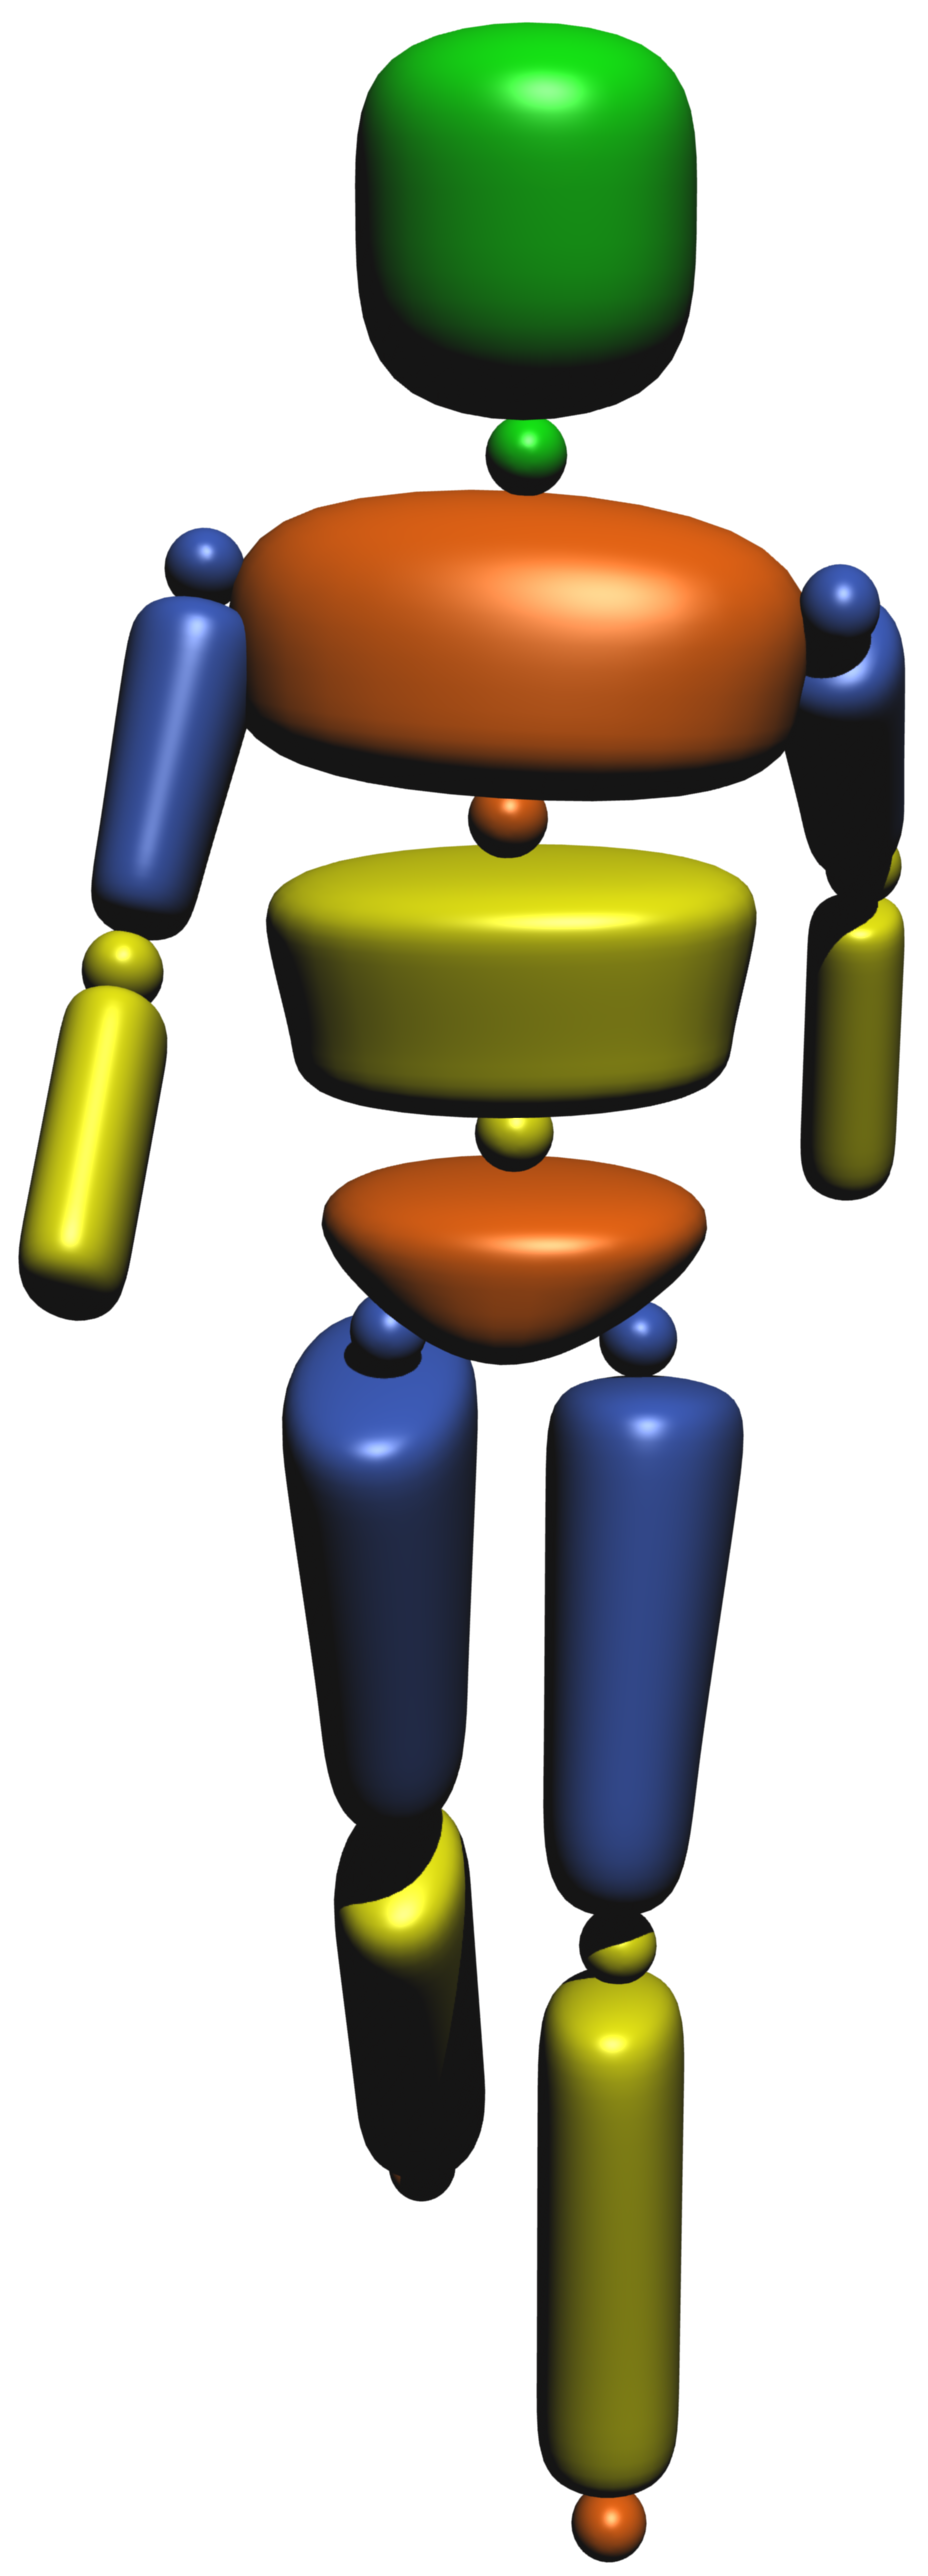
\includegraphics[width=0.1\textwidth]{fig/knubbi.png}
%   \caption{Example picture.}
%   \label{fig:knubbi}
%\end{figure}
%
%\subsection{Bibliography styles}
%The \texttt{orbref-num.bst} bibliography style numbers the citations by their order of appearance. Here are two sample references: \cite{Newton1687,Mombaur2009}.
%
%\subsection{Lorem Ipsum}
%\lipsum[1]
%
%%% Table
%\begin{table}[h]
%\caption{Example table.}
%   \begin{tabularx}{0.48\textwidth}{llr}
%   		 \toprule 
%   		 Symbol & \multicolumn{1}{X}{Description} & Value [m] \\
%		 \midrule
%		  $A_x$ & Horizontal coordinate of A$^{*}$ & 0.0745 \\
%		  $A_z$ & Vertical coordinate of A$^{*}$ & 0.2650 \\  \noalign{\smallskip}
%		  
%		  $C_x$ & Horizontal coordinate of C$^{\#}$ & 0.0700 \\
%		  $C_z$ & Vertical coordinate of C$^{\#}$ & 0.1000 \\
%		  $D_x$ & Horizontal coordinate of D$^{\dag}$ & 0.0602 \\
%		  $D_z$ & Vertical coordinate of D$^{\dag}$ & 0.0860 \\
%		 \bottomrule
%   \end{tabularx}  \label{tab:initmodel}
%\end{table}
%
%\lipsum[2]

\bibliography{mybibfile}

\end{document}
